%% Generated by scripts/build_manuscript.py from docs/paper/MANUSCRIPT.md -- do not edit.
\documentclass[referee,lineno,pdflatex,sn-basic]{sn-jnl}
\usepackage{graphicx,booktabs,tabularx,amsmath,amssymb,xcolor,tikz,url}
\renewcommand{\tabularxcolumn}[1]{>{\raggedright\arraybackslash}p{#1}}
\usetikzlibrary{arrows.meta,positioning,fit}
\raggedbottom
\begin{document}
\title[The Price of Utility]{The Price of Utility: Scientific Computation as Browser Admission Work, Measured Under Attack}
\author*[1]{\fnm{Rishi} \sur{D V}}\email{rishidv2005@gmail.com}
\author[1]{\fnm{Ram Ganesh} \sur{Vemula}}\email{ramganeshvemula@gmail.com}
\author[1]{\fnm{Sanjay} \sur{D M}}\email{sanjaydm23072005@gmail.com}
\author[1]{\fnm{Rithik Madhav} \sur{V}}\email{rithik7680@gmail.com}
\author[2]{\fnm{Jayashree} \sur{R}}\email{jayashree@pes.edu}
\affil*[1]{\orgname{PES University}, \orgaddress{\city{Bengaluru}, \state{Karnataka}, \country{India}}}
\affil[2]{\orgdiv{Department of Computer Science and Engineering (AI \& ML)}, \orgname{PES University}, \orgaddress{\city{Bengaluru}, \state{Karnataka}, \country{India}}}
\abstract{Proof-of-work admission spends client computation on puzzles. We investigate replacing that work with bounded AutoDock Vina searches whose outputs join a virtual-screening campaign. The evaluation combines molecular replay, phone measurements and admission simulations under a versioned protocol. Across five preselected 96-compound panels and 2,073 paired state jobs, decomposition changed mean ROC-AUC by $-$0.0008 to +0.0033; paired 95\% intervals lay within $\pm$0.017. Tested browser units reproduced reference pool and trace hashes. Committing to the trace rejected all 198 tested truncated-work submissions, whereas result-only commitments accepted some. Scheduler fixes removed large attacker discounts observed with free identities; remaining bundle-tier estimates were near parity under the evaluated cost model, without establishing a general work lower bound. Fabricated energies in 5\% of units worsened 22 of 33 re-finalised jobs. An exploratory resampling projection at 10\% corruption estimated ROC-AUC losses up to 0.034; rescoring before merge reduced this effect in the tested corpus. Phone measurements showed no general latency-variability advantage over a 64-subpuzzle baseline. Availability simulations expose the principal cost: a structurally admissible fake selected for audit consumes a molecular replay. We evaluate a conditional capacity model and a mock-attestation lane whose benefits depend on assumed issuer quotas and attacker token supply. Useful-work admission can preserve scientific screening performance on these panels, but trades cheap verification for replay capacity and imposes unequal costs across devices.}
\keywords{proof of work, useful work, admission control, CAPTCHA alternatives, volunteer computing, denial of service, result verification, molecular docking}
\maketitle

\section{Introduction}

Websites that cannot tell people from programs increasingly ask the visitor's browser to pay in computation. Proof-of-work CAPTCHAs, rate-limiting proxies against AI crawlers, and Tor's onion-service defence charge computation before admitting requests~\citep{Back02,FriendlyCaptcha,Anubis,TorPoW23}. Their puzzle constructions differ, but verification is much cheaper than solving and the output is not a scientific result. Fresh challenge binding limits answer reuse; admission still requires expiry, replay protection and a cost model.

This paper asks what the web gives up, and what it gains, when that discarded computation is replaced by computation someone needs. An admission in our system uses one or more bounded units of molecular docking with AutoDock Vina~\citep{Trott10,Eberhardt21}, and each accepted unit becomes part of a virtual screening campaign. The idea is not new. reCAPTCHA turned human admission effort into book digitisation~\citep{vonAhn08}, Coinhive turned browser admission into cryptocurrency mining~\citep{Rueth18}, and a recent design proposes cracking password hashes in place of hashcash~\citep{ChadamTopa23}. What has been missing is a measured answer to whether such a gate can be made secure, and at what cost.

Useful work changes both verification cost and answer reuse. Verifying a docking unit requires replay, far more expensive than checking a hash-puzzle solution. Scientific inputs may recur, so assignments and one-use credits must prevent repeated redemption of the same result. We investigate whether decomposition, trace commitment and sampled replay preserve useful output while removing exploitable discounts in admission cost. The tested fixes remove large observed discounts; they do not establish a lower bound against all algorithms, hardware or strategies. Replay capacity and device disparity remain material costs.

This paper is organised around one thesis: useful computation can replace discarded proof of work at a browser gate, but verification changes the economics of admission. We test it through five questions, each answered by a separate experiment under a protocol written before any attack was implemented. The protocol was amended twelve times, each amendment's predictions committed to version control before the experiment it governs, and every miss is reported. The measured answers are our contributions.

\begin{enumerate}
\item \textbf{Can a docking search be split into admission-sized units without changing the science?} On five qualified panels, screening results are preserved at matched evaluation counts (Section 5.1).
\item \textbf{Can browsers reproduce those units exactly?} Every tested unit on five phone models reproduced the reference output bit for bit; unit latency is as predictable as a 64-subpuzzle puzzle, not more (Section 5.2).
\item \textbf{Can clients fake the work cheaply?} Some strategies initially could. Trace commitment and three scheduler fixes remove the large measured discounts, leaving estimates near parity with free identities; no general lower bound is established (Sections 5.3 and 6).
\item \textbf{Can fabricated work corrupt the science without being admitted?} Yes, through the merge. Rescoring before merging mitigates the measured failure (Section 5.4).
\item \textbf{Is useful work better than proof of work?} Not universally. Replay turns fake submissions into verifier load, device disparity decides who is denied first, and an outside trust signal helps only under stated issuer assumptions (Section 5.5).
\end{enumerate}

We also report where the approach loses. A puzzle beats useful work on verifier cost and freshness, as predicted. Identity cost matters in ways it does not for proof of work. Availability under a sustained attacker with about 16 CPU cores is not solved by any configuration we tested, and the attestation that helps most is unavailable in Android browsers.

\section{Related work}

\subsection{Client puzzles and proof-of-work admission}

Charging a requester computation before granting a shared resource goes back to Dwork and Naor's pricing functions~\citep{DworkNaor92} and Back's Hashcash~\citep{Back02}. Juels and Brainard applied client puzzles to connection depletion~\citep{JuelsBrainard99}, already dividing a puzzle into independent subpuzzles, and Aura et al. combined puzzles with stateless authentication~\citep{Aura00}, as our ticket prototype does. Stebila et al. strengthened the definition of puzzle difficulty so that solving n puzzles is provably n times as hard as solving one~\citep{Stebila11}, which is the property our effort count, a number of distinct subpuzzle solutions, relies on. The property of puzzles we contrast with most is older and simpler: a hash puzzle verifies cheaply relative to solving, substantially reducing the verifier load per submission compared with molecular replay.

Two lines of criticism carry over directly. Laurie and Clayton argued that no single price deters spammers without burdening legitimate senders, because the two groups' computing resources differ too widely~\citep{LaurieClayton04}. Abadi et al. traced the same disparity to hardware and proposed memory-bound functions so that low-end and high-end machines pay similar costs~\citep{Abadi05}. Our device measurements show the disparity is sharper in browsers: native hashing runs about 36 times faster per core than the budget phone's JavaScript, and that ratio, not the price rule, decides which newcomers lose under attack. Liu and Camp answered Laurie and Clayton by weighting the work requirement with a reputation function~\citep{LiuCamp06}; our trust tier, earned by three audited bundles, and our attested lane are instances of that idea.

Proof of work has become a deployed browser defence. Friendly Captcha splits the work into many small puzzles to reduce solve-time variance~\citep{FriendlyCaptcha}, ALTCHA and mCaptcha offer self-hosted variants, the latter framed as a rate limiter rather than a human test~\citep{mCaptcha24}, and Anubis, released in 2025, places a SHA-256 challenge in front of sites to slow AI crawlers~\citep{Anubis}; operators report that crawlers adapted within months. NGCaptcha~\citep{Ding25} couples a hash puzzle with a visual task designed to resist vision models, and reasoning gates replace hashing with puzzles that are costly for AI agents to reason through yet cheap to check~\citep{Kumar25}; neither produces useful output. Among image and behavioural CAPTCHAs, Searles et al. measured 1,400 users solving deployed CAPTCHAs~\citep{Searles23}, and Motoyama et al. showed that human solving services price CAPTCHAs at a small fraction of a cent~\citep{Motoyama10}. We take from this work the baseline (a subpuzzle hash puzzle is the strongest wasteful comparator) and the device-disparity problem. We do not claim a new puzzle. On phones, a 64-subpuzzle puzzle proved as predictable as a docking unit (Section 5.2), so we claim no latency advantage over this baseline.

\subsection{Useful work in place of wasted work at the gate}

reCAPTCHA made the human effort spent at an admission gate useful by pairing an unknown word, whose transcription digitised books, with a control word of known answer that decided admission~\citep{vonAhn08}. Our design mirrors that split at the level of computation: the admission decision rests on a replayed unit, and the remaining units are accepted into the scientific pool unverified. The difference is that reCAPTCHA needed human consensus to trust the unknown word, whereas a docking unit can be replayed bit for bit.

Computational useful work at the gate has been proposed with far less evidence. The Coinhive proof-of-work CAPTCHA mined Monero for the site owner; measurement studies documented how the same scripts were used without consent~\citep{Eskandari18,Konoth18,Rueth18}, a history that makes consent and transparency first-order design requirements for any system that spends a visitor's CPU. The closest prior proposal to ours is Chadam and Topa's password-cracking CAPTCHA~\citep{ChadamTopa23}: the visitor brute-forces a range of candidate passwords against a stored hash, and progress is trusted when at least 51\% of a small group of visitors agree. It is a four-page work-in-progress design without implementation measurements, adversarial evaluation or device results, and its majority rule is exactly the redundancy that Sybil identities defeat~\citep{Douceur02}. Klarman et al.'s Webcoin rewards crowdsourced web indexing rather than hashing and states plainly the problem we quantify: unlike a nonce, useful output cannot be validated in nanoseconds, so only a fraction of it is verified~\citep{Klarman18}.

What we add is not the idea but the measured system: a real scientific workload (AutoDock Vina~\citep{Trott10,Eberhardt21} units of 256,000 evaluations), verified by deterministic replay rather than by majority, shown to reproduce monolithic screening results at matched compute on five targets, attacked under a predeclared protocol, and timed in two phone studies, including a five-device subpuzzle comparison.

\subsection{Proofs of useful work in consensus}

Proof-of-useful-work research asks when the work securing a blockchain can also be useful. Permacoin repurposes mining for archival storage~\citep{Miller14}; Ball et al. defined proofs of useful work for problems such as orthogonal vectors and later revised their definition after observing that the original admits a naive construction~\citep{Ball17,Ball18}; Ofelimos realises a provably secure longest-chain protocol whose puzzle is a doubly parallel local search~\citep{Fitzi22}; Komargodski and Weinstein obtain proofs of useful work for arbitrary matrix multiplication with 1 + o(1) overhead under hardness assumptions~\citep{Komargodski25}. Dotan and Tochner show that wasteless mining constrains which problems can be used at all~\citep{DotanTochner20}.

These works need what our setting does not: problems chosen or derived without a trusted party, hardness guarantees for adversarially chosen instances, and public verification. An admission gate has a trusted server that assigns the task and holds the verification key, so useful work can come from an ordinary scientific queue. Pass shows that, at equilibrium pricing, useful work does not lower the cost of attacking a proof-of-useful-work chain~\citep{Pass26}; our measurements instead test particular strategies and find near-parity estimates after fixing structural discounts, without a comparable proof. What the consensus setting teaches instead is the cost of verification. Luu et al.'s verifier's dilemma shows that when checking a computation is expensive, rational verifiers skip it~\citep{Luu15}. Our verifier cannot skip replay without admitting fabricated output, so the dilemma becomes a capacity limit: every fake submission costs a full replay, and spare replay capacity, which costs the defender real CPU, bounds who can be admitted under attack.

\subsection{Result verification in volunteer computing}

Volunteer computing has verified untrusted results for over two decades. BOINC uses replication with adaptive policies based on host history~\citep{Anderson20}; Sarmenta introduced spot-checking and credibility-based fault tolerance~\citep{Sarmenta02}; Golle and Mironov planted secret "ringers" whose images reveal lazy workers~\citep{GolleMironov01}; and Kondo et al. measured how often desktop-grid results are actually wrong~\citep{Kondo07}. Browser volunteer computing followed with Pando~\citep{LavoieHendren19} and JSDoop~\citep{Morell19}, and Webina runs AutoDock Vina itself in the browser through WebAssembly~\citep{Kochnev20}. Docking itself has run on volunteer machines before, in Docking@Home on BOINC~\citep{Estrada10}, among long-lived, credited volunteers rather than anonymous visitors. Outside volunteer computing, Tan et al. audit an untrusted web server by re-executing its requests and cut the cost of naive replay by deduplication~\citep{Tan17}; our verifier replays one sampled unit per bundle and faces the same trade-off between audit coverage and re-execution cost.

Our audit is a spot check in Sarmenta's sense, and we do not claim the audit mechanism as new. Volunteer platforms also face untrusted participants and cheap identities; our emphasis is admission value obtainable through short sessions, retries and trust transitions. We test those paths with identity cost set to zero. The observed large discounts disappear after fixes, while bundle-tier estimates remain consistent with parity rather than proving it. Replay also requires execution to be deterministic across platforms. WebAssembly specifies deterministic floating point except for NaN payloads~\citep{Haas17}; we observed all 68 phone units bitwise identical to native execution across iOS and Android, and confined the only cross-toolchain divergence to last-bit C runtime differences amplified by Monte Carlo search.

A separate issue arises when unverified candidate pools are merged before all search units are audited. In our corpus, fabricated energies at 5\% of units worsened 22 of 33 re-finalised jobs. A separate exploratory projection at 10\% corruption estimated AUC losses up to 0.034. Rescoring candidates before merge mitigated the measured ordering failure. We claim this empirical failure mode and repair in the Vina admission pipeline, not the invention of aggregate poisoning or a general integrity guarantee.

\subsection{Pricing admission under denial-of-service attack}

Several designs let clients bid for scarce service. Wang and Reiter's puzzle auctions let clients choose puzzle difficulty and serve the highest bids first~\citep{WangReiter03}; speak-up has clients pay in bandwidth~\citep{Walfish06}; Portcullis allocates connection-setup capacity by per-computation fairness~\citep{Parno07}; and Chakraborty et al. price jobs from an estimate of the honest workload so that the defender's cost grows more slowly than the attacker's~\citep{Chakraborty22}. The deployed descendant closest to our mechanism is Tor's onion-service defence (proposal 327, shipped in Tor 0.4.8 in 2023), in which clients attach Equi-X proofs of self-chosen effort, requests wait in an effort-ordered queue, and the service publishes a suggested effort that rises with backlog and decays when idle~\citep{TorProp327,TorPoW23}. Our effort-priority newcomer queue (amendment 9) adopts that design and makes no claim to it.

What differs is what the queue protects. In our design a structurally valid fake selected for audit consumes a molecular replay. We test the conditional budget scale (R $-$ $\lambda$) $\times$ device hash rate $\times$ patience, with R the verifier's replay rate and $\lambda$ the honest arrival rate. It models a full-patience honest bid and spare service capacity; it is not a universal admission threshold. Section 5.5 reports the original simulations separately from an exact-service, five-seed correction. Both use real queue code with modeled replay and puzzle costs rather than deployment traffic.

\subsection{Privacy-preserving attestation as an outside trust signal}

Privacy Pass lets a client that solved one challenge redeem unlinkable tokens later instead of solving more~\citep{Davidson18}; its architecture, HTTP scheme and issuance protocols, including publicly verifiable blind-RSA tokens, are now RFCs 9576--9578~\citep{RFC9576,RFC9577,RFC9578}. Apple's Private Access Tokens use this scheme with the device vendor as attester, and Cloudflare's Turnstile accepts them in place of a challenge~\citep{ApplePAT22,Turnstile22}. A draft that would let issuers cap tokens per client per origin~\citep{RateLimitDraft} expired in 2024. Apple states that its attester can rate-limit devices to detect farms but publishes no limits. On the web outside Apple platforms the equivalent is missing: Google's Web Environment Integrity proposal was abandoned in 2023~\citep{WEI23}, and Play Integrity attests Android apps rather than web pages~\citep{PlayIntegrity}. Scrappy combines direct anonymous attestation with hardware security devices to give servers unlinkable rate-assurance proofs~\citep{Akama24}, the closest research design to the per-device cap our lane assumes. Critics object to device attestation on openness grounds~\citep{Rescorla22}.

Our attested lane (amendments 10 and 12) models an application of rate-limited tokens, not a new credential or deployed issuer integration. A mock issuer stands in for origin-bound, single-use tokens and a per-device quota; blind signatures are not implemented. Simulations test whether a reserved lane can help token holders reach trust under CPU flooding, conditional on an externally constrained attacker token supply. Cheap attacker tokens can instead consume the protected replay capacity. The assumed per-device cap is not a published guarantee of deployed issuers. The platform literature therefore motivates an assumption to test, not a demonstrated deployment path for every browser or budget phone.

\subsection{Scientific workload}

AutoDock Vina~\citep{Trott10} and its 1.2 release~\citep{Eberhardt21} are among the most widely used docking programs, and large-scale docking is a standing demand for computation. We make no methodological claim about docking. Our scientific claim is narrow: decomposing an exhaustiveness-32 search into independent 256k-evaluation units and merging them with Vina's own finaliser changed mean screening ROC-AUC by $-$0.0008 to +0.0033, with paired 95\% intervals contained within $\pm$0.017, on five 96-compound panels at under 0.5\% extra evaluations.

---

\section{System and threat model}

\subsection{Workload and decomposition}

The scientific workload is structure-based virtual screening with AutoDock Vina 1.2.7. A Vina docking run at exhaustiveness 32 performs Monte Carlo searches with local BFGS refinement and merges their minima through a finaliser that clusters and refines the best candidates. We split each run into independent units of 256,000 energy evaluations, each with its own server-assigned seed, and merge the units' minima pools with Vina's original finaliser (Figure 1). A ligand state requires a median of 140 units. Units are the admission currency: a visitor's browser runs one or more units in WebAssembly and uploads the resulting minima pool.

Prepared receptor and grid state is delivered through a content-addressed CDN, so a warm browser runs a unit in about 2 s on a current phone and 7.5 s on a 2019 budget phone (Section 5.2).

\begin{figure}[htbp]
\centering
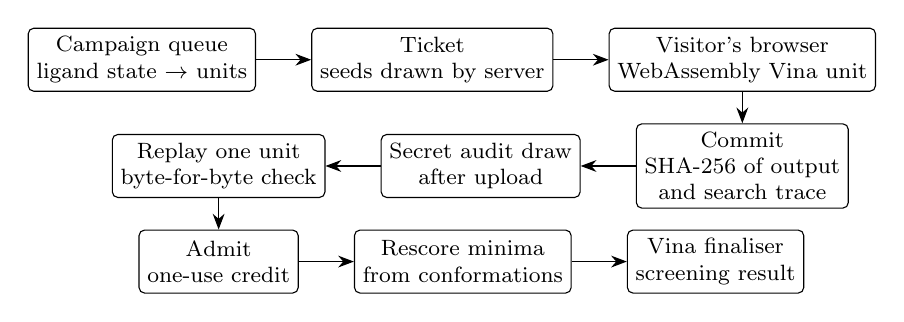
\begin{tikzpicture}[font=\footnotesize,node distance=4mm and 7mm,
  box/.style={draw,rounded corners=2pt,align=center,minimum height=8mm,inner sep=3pt},
  arr/.style={-{Stealth[length=2mm]}}]
\node[box] (queue) {Campaign queue\\ligand state $\rightarrow$ units};
\node[box,right=of queue] (ticket) {Ticket\\seeds drawn by server};
\node[box,right=of ticket] (browser) {Visitor's browser\\WebAssembly Vina unit};
\node[box,below=of browser] (commit) {Commit\\SHA-256 of output\\and search trace};
\node[box,left=of commit] (draw) {Secret audit draw\\after upload};
\node[box,left=of draw] (replay) {Replay one unit\\byte-for-byte check};
\node[box,below=of replay] (admit) {Admit\\one-use credit};
\node[box,right=of admit] (rescore) {Rescore minima\\from conformations};
\node[box,right=of rescore] (final) {Vina finaliser\\screening result};
\draw[arr] (queue)--(ticket);\draw[arr] (ticket)--(browser);\draw[arr] (browser)--(commit);
\draw[arr] (commit)--(draw);\draw[arr] (draw)--(replay);\draw[arr] (replay)--(admit);
\draw[arr] (admit)--(rescore);\draw[arr] (rescore)--(final);
\end{tikzpicture}
\caption{Admission with useful work. The server assigns units with fresh seeds; the browser runs one or more units and commits to their outputs and search traces before learning which unit will be replayed; a secretly drawn unit is replayed exactly; accepted units are rescored and merged by Vina's own finaliser.}
\label{fig:system}
\end{figure}

\subsection{Verification}

Verification is replay. The server re-executes a sampled unit with the same build, inputs and seed and compares output byte for byte. Three measures make that comparison meaningful.

\begin{itemize}
\item \textbf{Output commitment.} A client commits to the SHA-256 of its full output before the audit draw is derived, and the draw is computed server-side from a secret, so a client cannot learn which unit will be replayed before uploading.
\item \textbf{Trace commitment.} The commitment covers a hash of the per-step search trace, not only the final minima pool. Section 5.3 shows why the pool alone is insufficient.
\item \textbf{Fresh seeds.} Each unit's seed is drawn by the server, and a unit re-issued after expiry or failure receives a new seed, so an earlier answer cannot satisfy that new assignment. This prevents ordinary duplicate-answer caching, not every form of precomputation or algorithmic shortcut.
\end{itemize}

Build equivalence was established before any security experiment: three builds from the same sources and flags agreed coordinate for coordinate with an uninstrumented reference on every retained pose, and divergence from the official prebuilt binary was confined to last-bit C runtime differences amplified by Monte Carlo search.

\subsection{Admission tiers}

Newcomers are admitted in bundles of four units, one of which is replayed, so verifier cost is 25\% of client work at one audit draw. An identity that has had three bundles replayed and accepted may enter a trusted tier in which units are audited at a rate p. Each admission grants one single-use credit.

For availability we evaluate, as isolated prototypes rather than the deployed scheduler, stateless authenticated tickets with reserved capacity for established users, an effort-priority queue for newcomers adopted from Tor's onion-service defence~\citep{TorProp327}, and an attested lane for newcomers holding token from a mock issuer inspired by Privacy Pass~\citep{Davidson18,RFC9576}. The mock assumes an origin-bound, single-use token with a per-device quota; it does not implement blind signatures or integrate a deployed issuer.

\subsection{Threat model}

Identities are free. The attacker knows the protocol, submits arbitrary bytes, keeps anything it has computed, coordinates across identities and may hold native CPU cores. It cannot forge server commitments or read server secrets. Trust grants and replay verdicts come from trusted server components. We evaluate eight attacker behaviours, fixed in the protocol before any was implemented: zero work (A1), partial work (A2), cached replay (A3), retry grinding (A4), identity reset (A5), disappearing workers (A6), collusion (A7) and subtle scientific corruption (A8). A8 distinguishes useful work from puzzles, because a plausible but wrong result cannot be rejected by a cheap structural check. Attacks on the verifier's host, side channels and compromise of the attestation issuer are out of scope.

\section{Methodology}

\subsection{Predeclared protocol}

The evaluation follows a written protocol dated 22 September 2026, before any attack was implemented and before the matched scientific campaign completed. Thresholds could not be revised after outcomes were seen; every change is a dated amendment committed to version control before the experiment it governs, with the original preserved. Twelve amendments cover phase operationalisation, the three economic fixes, scientific integrity, trace commitment, the rescoring driver, newcomer pricing, attestation and the subpuzzle baseline, and a post-review replay-timing correction with five-seed replication. Where a prediction failed we report the failure, its cause and any post-hoc diagnostic separately from the predeclared result.

\subsection{Corpus, manifests and statistics}

Attacks run on real molecular output, not synthetic records. The corpus is the set of campaign jobs whose salted hash falls below 5\% of the hash space, a rule fixed before any attack was designed; 33 jobs across all five targets were recovered, containing 4,397 units with raw minima pools, traces and metrics. Every run writes a frozen execution manifest recording protocol, corpus, build and runner hashes, and re-running with a changed input fails. Proportions are reported with exact (Clopper--Pearson) 95\% intervals. Attacker discount factors are ratios of attempt counts; we report 95\% intervals from the geometric distribution of attempts per admission, treating attempts as independent.

\subsection{Measurement boundaries and reproducible methods}

\begin{table}[htbp]
\caption{Evidence supporting the claims and what each experiment does not establish.}
\centering
\small
\begin{tabularx}{\textwidth}{XXX}
\toprule
Claim & Evidence & Boundary \\
\midrule
Screening preservation & Actual native paired docking and finalisation, five panels & Qualified 96-compound panels, not full libraries or prospective biological validation \\
Trace-bound replay & Actual unit re-execution and byte/hash comparison & Tested builds, inputs and attacks; not a computational lower bound \\
Admission economics & Committed scheduler with simulated time and replay-derived verdicts & Specified strategies and cost model; not production traffic \\
Scientific poisoning & Actual corpus re-finalisation; separately, score-shift resampling & Whole-panel AUC effects are exploratory projections \\
Browser feasibility & Real phone execution and reference hash checks & Cooperative sessions, selected repeated units; not client attestation \\
Overload and trust bootstrap & Real queue SQL with modeled arrivals, replay and puzzle costs & Conditional finite-horizon simulations; not measured HTTP throughput \\
Attestation benefit & Mock issuer, token checks and one-use nullifiers & Assumed quota and token supply; no deployed issuer or blind-signature integration \\
\botrule
\end{tabularx}
\end{table}

Supplementary Section S1 gives the complete protocols: target selection and input preparation, compute matching and the paired bootstrap, the poisoning projection, and the availability simulator. The availability results use exact replay-event timing and five seeds (amendment 12). That amendment corrected an earlier discretisation which, by noticing completions only on 250 ms ticks, lengthened each simulated 1.52 s replay to 1.75 s; the original single-seed results are preserved and compared in Supplementary Section S3.

\subsection{Use of AI tools}

Large language model coding assistants (Anthropic Claude and OpenAI Codex) were used to implement experiment code, analysis scripts and prototypes, to search and verify literature, and to draft text, under the author's direction. All predictions were committed to version control before the experiments they govern ran; every number in this paper is produced by committed scripts from recorded data; and the author reviewed the code, results and text and takes responsibility for them. The assistants are not authors.

\section{Results}

\subsection{Can docking be decomposed without changing the science?}

Five targets from the DUD-E benchmark~\citep{Mysinger12}, selected from published Vina results before any local run and each a panel of 32 actives and 64 decoys, passed predeclared ranking and redocking gates with stock Vina (ROC-AUC 0.87--0.99). In a matched comparison of 2,073 paired state jobs over three seeds with no failures, every ligand state was docked both as one exhaustiveness-32 run and as independent units merged by the original finaliser, at matched evaluation budget.

\begin{table}[htbp]
\caption{Matched comparison of decomposed and monolithic docking: change in screening ROC-AUC, three seeds, 96-compound panels.}
\centering
\small
\begin{tabularx}{\textwidth}{XrXr}
\toprule
Target & Mean $\Delta$AUC & Paired 95\% interval & Evaluation ratio \\
\midrule
WEE1 & $-$0.0003 & [$-$0.0015, +0.0000] & 1.0040 \\
PUR2 & +0.0033 & [$-$0.0067, +0.0164] & 1.0025 \\
FA7 & +0.0020 & [$-$0.0093, +0.0163] & 1.0034 \\
TGFR1 & $-$0.0008 & [$-$0.0060, +0.0036] & 1.0045 \\
KIF11 & +0.0003 & [$-$0.0042, +0.0049] & 1.0045 \\
\botrule
\end{tabularx}
\end{table}

Every interval lies within $\pm$0.017 and straddles or touches zero; EF10 was identical on 14 of 15 target--seed pairs. Decomposition costs under 0.5\% extra evaluations and no extra search time. The predeclared non-inferiority margin of $-$0.05 is generous relative to these effects, so we read the result from the intervals, not the margin. These are 96-compound panels, not full-library screens.

\subsection{Can browsers reproduce the units, and at what latency?}

In a first study on four phones, every one of 68 units was bitwise identical to the native reference output across iOS and Android. Against a single hashcash puzzle calibrated on each device to its median unit, 21.9\% of puzzle solves exceeded twice the median and none of 64 warm units did (Supplementary Section S2). Natively, a docking unit also had half the coefficient of variation of a median-matched hashcash puzzle (0.48 against 0.95).

A single hash puzzle is not the strongest baseline: deployed proof-of-work CAPTCHAs split the work into many small puzzles~\citep{FriendlyCaptcha}, and the sum of 64 geometric solve counts is far narrower than one. We therefore ran a second page on five phones, interleaving each unit with two single puzzles and two 64-subpuzzle puzzles, all calibrated on the device to its median unit (amendment 11).

\begin{table}[htbp]
\caption{Five phones, 16 warm units and 24 solves of each puzzle type per phone, pooled by each device's median unit time as predeclared.}
\centering
\small
\begin{tabularx}{\textwidth}{Xrrr}
\toprule
Kind & n & p95/median & Over 2$\times$ median \\
\midrule
Docking unit & 80 & 1.15 & 0\% \\
Single puzzle & 120 & 4.40 & 25.8\% \\
64-subpuzzle puzzle & 120 & 2.02 & 5.8\% \\
\botrule
\end{tabularx}
\end{table}

Two of four predictions held: single puzzles again had a long tail, and units stayed within 1.35 times their median at the 95th percentile. The prediction that subpuzzles would too failed, and so did the calibration check that explains it: on-device calibration missed by up to a factor of 1.66 (Moto Edge 50) and 0.70 (Galaxy M30s), so pooling by unit time mixes shifted distributions. Measured within each device instead, a post-hoc analysis, subpuzzle solves had p95/median 1.14--1.40 and none exceeded twice their own median; pooled, 1.21 against 1.15 for units (Figure 2). As stated before the experiment, lower latency variance is therefore not an advantage of useful work over a well-designed puzzle. It is an advantage only over a single puzzle.

\begin{figure}[htbp]
\centering
\includegraphics[width=0.6\textwidth]{figures/device_latency.pdf}
\caption{Solve time on five phones for docking units, single puzzles and 64-subpuzzle puzzles run in the same sessions. Each time is divided by its device's median for that kind, so the curves compare distribution shape; the dotted line marks twice the median. Calibration error, which this scaling removes, is reported in the text.}
\label{fig:latency}
\end{figure}

The budget phone is 3.7 times slower than the iPhone at docking but 5.2 times slower at JavaScript hashing, and its first contribution takes about 13 s including asset delivery, a real accessibility cost.

All 85 units in this second study also matched the reference output exactly.

\subsection{Can clients fake the work cheaply?}

\textbf{Unit-level attacks under real replay.} We ran 693 trials on 99 units sampled by salted hash from the corpus, across all five targets.

\begin{table}[htbp]
\caption{Unit-level attacks judged by exact replay, 99 corpus units.}
\centering
\small
\begin{tabularx}{\textwidth}{XrX}
\toprule
Attack & Accepted & 95\% interval \\
\midrule
Honest unit & 99/99 & [0.96, 1.00] \\
A1 substitution of another unit's result & 0/99 & [0.00, 0.04] \\
A3 cached resubmission & 99/99 & by design; one-use credits refuse it \\
A2 quarter work, pool-only commitment & 20/99 & [0.13, 0.30] \\
A2 half work, pool-only commitment & 45/99 & [0.35, 0.56] \\
A2 quarter or half work, pool and trace commitment & 0/198 & [0.00, 0.02] \\
\botrule
\end{tabularx}
\end{table}

Committing to the minima pool alone does not enforce work: the retained minima of a Vina search often stabilise before its budget is spent, so a search stopped at a quarter or half of its evaluations can reproduce the full pool byte for byte. Binding the per-step trace rejected every tested quarter- and half-budget submission. This tests those truncation strategies, not a general computational lower bound. Hashing the trace preserves the tested replay check, subject to collision resistance, while cutting median upload from 163 KB to 19 KB. Falsifying the best energy by 0.1--3.0 kcal/mol never changed any output, because the finaliser recomputes energies; moving the best pose by 0.1 or 0.5 \AA{} had no effect.

\textbf{Admission economics with free identities.} We define the attacker discount factor as attacker work per admission divided by honest work per admission in the same tier. A hash puzzle is normalised to 1.0 under a common hardware and expected-hash cost model; that is not a claim of equal wall time or energy across hardware. Below 1.0, the modeled attacker cost is lower than the honest cost. On the committed scheduler, 118 configurations were run with audit verdicts resampled from real replay records.

As first built, the scheduler had three flaws. Abandoned units returned with the same seed, so an attacker who computed one of four units reused it until the audit draw landed on it. The audit draw was revealed before upload, so a trusted identity could abandon exactly when selected and never be caught. And trust was granted after one bundle. Each fix was predeclared and measured separately.

\begin{table}[htbp]
\caption{Attacker discount factor on the committed scheduler before and after the three fixes.}
\centering
\small
\begin{tabularx}{\textwidth}{XrXX}
\toprule
Configuration & Before & After, 95\% interval & Predicted \\
\midrule
Bundle tier, attacker computes 1 of 4 units & 0.46 & 0.96 $\pm$ 0.09 & 0.95--1.10 \\
Bundle tier, attacker computes 2 of 4 units & 0.57 & 1.03 $\pm$ 0.08 & 0.95--1.10 \\
Bundle tier, attacker computes 3 of 4 units & 0.76 & 1.00 $\pm$ 0.06 & 0.95--1.10 \\
Trusted tier, trust after 1 bundle, p = 0.02--0.25 & 0.44--1.19 & 0.44--1.40, reveal removed & analytic, matched \\
Trusted tier, trust after 3 audited bundles & --- & 1.36--4.04 & at least 1.0 \\
\botrule
\end{tabularx}
\end{table}

With reseeding, no reveal and a three-bundle threshold, the large observed bundle-tier discounts (0.46--0.76) disappear: tested estimates become 0.96--1.03. These are consistent with parity under the evaluated cost model. The lowest interval, 0.96 $\pm$ 0.09, also permits a modest attacker advantage; containing 1.0 does not establish equality or a lower bound of 1.0. The trusted-tier strategies tested after the threshold change cost 1.36--4.04. Identities are free in these experiments, but results apply to the specified strategies, attempt model and workload costs, not every possible adversary. Before the fixes, compensating for the measured discounts would have required an identity price of 0.5--5.1 honest units. The fixes remove the particular reuse, disclosure and early-trust paths responsible for those discounts.

Capacity exhaustion by workers who accept units and disappear behaved as a threshold rather than proportionally: holders of 4, 8 and 12 of 16 leases caused no refusals, and 16 caused 81\%. Stateless tickets that allocate seeds without reserving queue seats removed the effect in the isolated prototype.

Section 6 discusses what trace commitment does and does not establish about the work an accepted unit requires.

\subsection{Can fabricated work corrupt the science?}

An attacker need not be admitted to harm the campaign; it need only place units in the pool. We ran the original finaliser over the corpus with units replaced or altered.

\begin{table}[htbp]
\caption{Corpus re-finalisation measurements; the ROC-AUC entry is a separate exploratory projection.}
\centering
\small
\begin{tabularx}{\textwidth}{XX}
\toprule
Experiment & Measured \\
\midrule
Units with the wrong atom count & rejected 33/33 \\
Honest duplication of 5--75\% of units & measured best gain $-$0.10 kcal/mol; projected ROC-AUC within $\pm$0.004 up to 25\% \\
Duplicated units claiming $-$20 kcal/mol, 5\% of units & 22 of 33 jobs worse (95\% interval 0.48--0.82), by up to 2.6 kcal/mol \\
\botrule
\end{tabularx}
\end{table}

No falsified energy ever reached output: the finaliser recomputes every reported energy. But its merge still ranks and clusters minima by the energies clients report and keeps a bounded set for refinement, so fabricated minima displace honest ones before refinement sees them. In an exploratory, non-predeclared resampling projection, mean ROC-AUC changes reached about $-$0.016 at 5\% and $-$0.034 at 10\% fabricated units. These are not measured whole-panel poisoning outcomes: corpus score shifts were resampled onto otherwise unchanged campaign scores (Supplementary Section S1). A revised driver that rescores every submitted minimum from its conformation before merging was verified against the same gates.

\begin{table}[htbp]
\caption{Rescoring driver against the original driver.}
\centering
\small
\begin{tabularx}{\textwidth}{XXX}
\toprule
Check & Original & Rescoring \\
\midrule
Build-equivalence gates and replay, five targets & pass & pass \\
Honest pools finalised & --- & byte-identical, 33/33 \\
Falsified-energy attack, projected mean $\Delta$AUC & as low as $-$0.034 & within $\pm$0.0016 \\
Jobs worsened at 5\% falsified units & 22/33 & 2/33, as honest duplication \\
Rescoring overhead per ligand state & --- & +91 ms median; 0.046\% relative to calibrated client work \\
\botrule
\end{tabularx}
\end{table}

The original driver is retained as the historical baseline for every earlier result. The relative overhead denominator is number of units multiplied by a calibrated 1,520 ms per unit, not measured client time for each attacked job. The $\pm$0.0016 AUC range is also a projection. Rescoring addresses fabricated energy ordering; it does not certify that unaudited pools contain all minima that honest search would have found.

\subsection{What does useful work cost compared with proof of work?}

A hashcash puzzle calibrated natively to a similar median client time (1.38 s against 1.52 s for a unit) verifies in 0.77 $\mu$s. Verifying useful work costs a replay of 1.52 s for each audited unit, a fraction q of client work: about five orders of magnitude more at q = 0.1. The puzzle also guarantees freshness, which useful work must restore with assignment seeds and one-use credits. The rest of this section asks what that verification cost does under attack.

A structurally admissible fake selected for audit consumes a modeled 1.52 s replay, whereas hash-puzzle verification is comparatively cheap. Let R be replay service capacity, $\lambda$ the honest newcomer arrival rate, r a device's hash rate and T its bidding budget. Under full-patience bidding, an honest bid is approximately rT hashes. Buying the spare R $-$ $\lambda$ replay slots per second at that price gives the budget scale (R $-$ $\lambda$) $\cdot$ r $\cdot$ T. This is a conditional capacity model, not a universal threshold: finite queues, transient prices, device mixtures, randomized solve times and the attack/drain horizon can change observed service. The predeclared C1 test checks only budgets below half or above twice this scale, leaving the intermediate band untested.

\textbf{Historical results and correction.} The original follow-price experiment passed 33/48 C1 checks; the full-patience follow-up passed 46/48. Both used one seed and rounded replay completion to the next 250 ms tick, giving 1.75 s service rather than the assumed 1.52 s. Amendment 12 preserves those results and repeats all four grids with exact replay events and five seeds, 1,120 runs in total. The corrected full-patience experiment passes 230/240 eligible checks: 46/48 in each seed. The same two directional misses recur at one worker: budget-phone service at 0.1 attacker cores and flagship service at one core exceed the predicted upper limit. These are not 240 independent traffic scenarios or validation of an exact cutoff (Figure 3).

Supplementary Table S2 lists every prediction check, original and corrected.

At eight replay workers the priority mechanism still discriminates sharply by device under a four-core attack. Corrected service means are 0.070, 0.965 and 1.000 for budget, mid-range and flagship devices. At sixteen attacker cores they are 0.110, 0.135 and 0.130. Service is measured within the finite observation window, including post-attack draining; it is not a ten-second admission guarantee.

\begin{figure}[htbp]
\centering
\includegraphics[width=\textwidth]{figures/served_vs_cores.pdf}
\caption{Corrected full-patience simulation: mean service across five seeds, with shading for the observed minimum--maximum range. Dashed lines mark the conditional budget scale $(R-\lambda)\,r\,T$, not a guaranteed cutoff. Input polling remains discrete; replay completion uses exact event times.}
\label{fig:served}
\end{figure}

A native core's measured hash rate is about 36 times the budget phone's JavaScript rate. Pricing alone does not remove that disparity. Under the sixteen-core bootstrap attack, without attestation, no budget or mid-range users reach trust in the corrected runs; flagship users reach trust at a mean of 0.030 (range 0--0.050) with eight workers. The historical single-seed statement that no device class ever reached trust is therefore too strong.

\textbf{Conditional mock-attestation result.} If an issuer supplies origin-bound, one-use tokens with an effective per-device quota, a separate replay lane can help token holders earn trust without winning the hash auction. This is an experiment with MockAttester, not a deployed Privacy Pass integration. At an assumed 90\% honest token coverage, every attested group reaches trust in all five seeds at attacker supply 0, 0.1 or 1 tokens/s with eight workers. At zero attacker tokens, mean within-seed median trust times are about 66 / 23 / 23 s, conditional on success and excluding the initial bundle's molecular work, which is already available at first arrival in this harness. Later bundles include device-calibrated work time. At ten attacker tokens per second, trust fractions fall and vary across seeds and device classes (Supplementary Table S4).

\begin{figure}[htbp]
\centering
\includegraphics[width=\textwidth]{figures/trust_bootstrap.pdf}
\caption{Corrected mock-attestation simulation under sixteen attacker cores. Bars show five-seed mean trust fractions; whiskers show observed minimum--maximum ranges. Left of the grey line: no attestation. Right: 90\% honest token coverage as assumed attacker token supply rises. The issuer and token-acquisition budgets are modeled.}
\label{fig:trust}
\end{figure}

A1, A3, A4 and A6 pass every corrected eligible check; A2 and A5 retain misses. The original post-hoc drain diagnostic and saturation failures remain in the archive. One-shot traffic drains after attack cessation; bootstrap attacks continue throughout the observation window, with repeated attempts until three grants. Consequently, one-shot service ratios and eventual trust fractions answer different questions. Token availability and issuer quotas are assumptions, and cheap attacker tokens consume capacity ahead of anonymous users. No conclusion here establishes production availability or an implementable quota from a deployed issuer.

\section{Discussion}

\textbf{When is useful work worth it?} Only when someone needs the output and the verifier can afford replay. A puzzle is strictly better on verifier cost and freshness. Useful work removes large observed attacker discounts only after closing the tested reuse and trust leaks, it is no more predictable for the visitor than a subpuzzle puzzle, and it pays in replay CPU for every fake submission. What it buys is that the visitor's computation is not wasted: the units a site would otherwise discard dock real ligands with screening differences small on the five qualified panels, within the reported uncertainty.

\textbf{What trace commitment does and does not establish.} The committed trace records, for every Monte Carlo step, the refined candidate's energy at full double precision and the cumulative number of energy evaluations. A matching trace therefore fixes the exact sequence of evaluations the honest algorithm performs, and replay compares it byte for byte. Two routes to a cheaper accepted trace remain open. Faster hardware or a faster implementation of the same operations, such as native code, vectorisation or a GPU, is not a shortcut in the security sense: it is the same hardware disparity proof of work already has, and Section 5.5 prices it. Avoiding evaluations is the real question. Approximate energies, reordered arithmetic or incremental updates change floating-point rounding and hence the committed bytes; fresh server-drawn seeds make one unit's intermediate states unlikely to recur in another. We know of no method that yields a matching trace with fewer evaluations than the honest search, but we have not proved that none exists. A lower bound of that kind, for example showing that any accepted trace of N steps requires $\Omega$(N) evaluations under stated assumptions about the scoring function, remains open.

\textbf{Identity cost.} Proof of work is indifferent to identities. Our first scheduler was not: its security depended on identities costing between 0.5 and 5.1 honest units. We regard this as the most transferable lesson for any useful-work admission design, whatever the workload: every retry, reveal and trust path must be checked with identities priced at zero.

\textbf{Availability.} The conditional budget scale (R $-$ $\lambda$) $\cdot$ r $\cdot$ T exposes the cost of replay capacity under the modeled attack. Corrected five-seed results retain substantial anonymous-newcomer denial at sixteen attacker cores. A mock-attestation lane improves outcomes only under assumed honest coverage and attacker token budgets; issuer quotas and platform availability remain external requirements, not properties established by our prototype.

\textbf{Consent.} Browser mining without consent became a documented abuse~\citep{Eskandari18,Konoth18}. A useful-work gate spends visitors' energy; it must say so, and it gives them a reason a puzzle cannot.

\textbf{Limitations.} Five phone models, one workload and five 96-compound panels. Availability mechanisms are isolated prototypes, not integrated into the deployed scheduler, and their puzzle costs were accounted from measured rates rather than executed. Discount-factor intervals assume independent attempts. The trusted tier grants unaudited admissions on history, not on the unit. Scientific quarantine after late detection is not implemented. The rescoring driver is a verified candidate, not yet serving traffic. Pool poisoning AUCs are projections based on exchangeable corpus score shifts. The availability replication measures five-seed variability but keeps arrival rates, device speeds, replay cost and attacker strategies fixed. Puzzle RNGs are seeded; prototype ticket identifiers and their tie-breaking remain cryptographically random. The initial bootstrap bundle is assumed ready at arrival. There is no integrated production traffic or energy-cost validation.

\section{Conclusion}

Useful computation can stand in for discarded proof of work at a browser gate, but verification changes the economics of admission. On five qualified panels, bounded Vina units preserve screening performance and reproduce exactly on phones. Trace commitment, fresh assignment seeds, concealed audit draws and a trust threshold remove the large discounts found in tested attacks; the remaining estimates are near parity under the cost model, not a proof that cheating cannot be cheaper. Rescoring mitigates a measured merge failure. Verification still consumes replay capacity, overload falls unequally on devices, and any benefit from external attestation depends on issuer and token-supply assumptions. These results quantify the practical costs and limits of useful-work admission rather than establish a universal replacement for proof of work.

\backmatter
\section*{Declarations}

\paragraph{Supplementary information}

Additional file 1 (PDF): Supplementary Information. Complete experimental methods (S1), the first four-phone timing study (S2), and all availability prediction checks, five-seed service and trust tables and historical comparisons (S3).

\paragraph{Availability of data and materials}

Project name: Capstone useful-work admission research prototype. Project home page: \url{https://github.com/Rishi94523/Capstone}. Archived version: [TODO: Zenodo DOI of the submission commit and result bundle]. Operating systems: Windows, Linux, and iOS and Android browsers. Programming languages: Python, C++, JavaScript and WebAssembly. Licence: MIT; AutoDock Vina and other upstream components, fetched and patched at build time rather than redistributed, keep their own licences (Vina: Apache 2.0). Protocol amendments, runners, manifests, analysis scripts and the figure and manuscript builders are in the repository.

\paragraph{Ethics approval and consent to participate}

Not applicable. All phone timing tests were run by the authors on phones they own. The test page submitted the device model and operating system as entered, the browser user agent and performance measurements; the study stored no names, contact details or location data.

\paragraph{Competing interests}

The authors declare that they have no competing interests.

\paragraph{Funding}

Not applicable.

\paragraph{Authors' contributions}

RDV conceived and designed the study, implemented the system, ran the experiments, analysed the results and wrote the manuscript. RGV, SDM and RMV ran the device experiments and reviewed and edited the manuscript. JR supervised the work and revised the manuscript. All authors read and approved the final manuscript.

\paragraph{Acknowledgements}

Not applicable.

\bibliography{references}
\end{document}
